\documentclass[tikz,border=2pt]{standalone}
\usepackage{pgfplots}
\pgfplotsset{compat=1.18}

\begin{document}
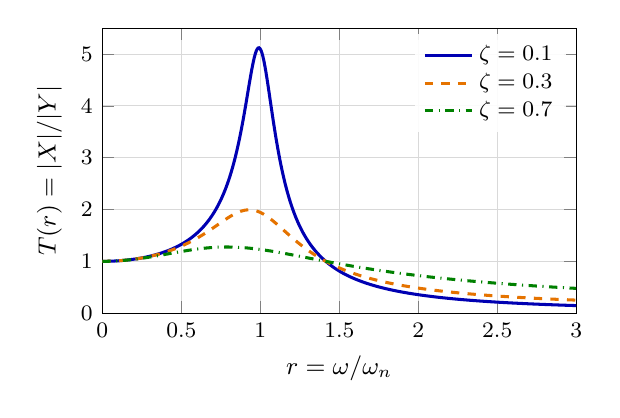
\begin{tikzpicture}
\begin{axis}[
    width=7.6cm,
    height=5.2cm,
    xmin=0,
    xmax=3,
    ymin=0,
    ymax=5.5,
    xlabel={$r=\omega/\omega_n$},
    ylabel={$T(r)=|X|/|Y|$},
    xtick={0,0.5,1,1.5,2,2.5,3},
    ytick={0,1,2,3,4,5},
    grid=both,
    major grid style={draw=gray!30},
    tick label style={font=\footnotesize},
    label style={font=\small},
    legend style={
        at={(0.98,0.98)},
        anchor=north east,
        draw=none,
        fill=white,
        fill opacity=0.9,
        text opacity=1,
        font=\footnotesize,
        row sep=-1pt
    }
]
\addplot[
    blue!70!black,
    line width=1.1pt,
    domain=0:3,
    samples=500
] {sqrt((1+(2*0.1*x)^2)/((1-x^2)^2+(2*0.1*x)^2))};
\addlegendentry{$\zeta=0.1$}

\addplot[
    orange!90!black,
    dashed,
    line width=1.1pt,
    domain=0:3,
    samples=500
] {sqrt((1+(2*0.3*x)^2)/((1-x^2)^2+(2*0.3*x)^2))};
\addlegendentry{$\zeta=0.3$}

\addplot[
    green!50!black,
    dashdotted,
    line width=1.1pt,
    domain=0:3,
    samples=500
] {sqrt((1+(2*0.7*x)^2)/((1-x^2)^2+(2*0.7*x)^2))};
\addlegendentry{$\zeta=0.7$}
\end{axis}
\end{tikzpicture}
\end{document}
